\documentclass[12pt,a4paper]{article}
\usepackage[utf8]{inputenc}
\usepackage{transparent}
\usepackage{amsmath}                                 % AMS Math Package
\usepackage{amsthm}                                  % Theorem Formatting
\usepackage{amssymb}                                 % Math symbols such as \mathbb
\usepackage{graphicx}                                % Allows for eps images
\usepackage[dvips,margin=1in,bottom=1in]{geometry}
\usepackage{mathtools}
\usepackage{tcolorbox}
\usepackage[explicit,compact]{titlesec}
\usepackage{csquotes}
\usepackage{booktabs}

\titlespacing\section{0pt}{12pt plus 4pt minus 2pt}{0pt plus 2pt minus 2pt}
\titlespacing\subsection{0pt}{12pt plus 4pt minus 2pt}{0pt plus 2pt minus 2pt}
\titlespacing\subsubsection{0pt}{12pt plus 4pt minus 2pt}{0pt plus 2pt minus 2pt}

\newcommand{\V}[1]{\ensuremath{\mathbf{#1}}} % vektor
\newcommand{\gv}[1]{\ensuremath{\mbox{\boldmath$ #1 $}}} 
\newcommand{\abs}[1]{\left| #1 \right|}                   % abslouttverdi
\newcommand{\avg}[1]{\left\langle #1 \right\rangle}       % gjennomsnitt

\newcommand{\der}[2]{\frac{\text{d} #1}{\text{d} #2}}     % derivert
\newcommand{\dd}[2]{\frac{\text{d}^2 #1}{\text{d}#2^2}}   % dobbelderivert
\newcommand{\pd}[2]{\frac{\partial #1}{\partial #2}}      % partiellderiverte
\newcommand{\pdd}[2]{\frac{\partial^2 #1}{\partial #2^2}} % doble partiellderiverte

% document layout

\setlength{\parindent}{0em}
\setlength{\parskip}{1em}
\setlength{\parindent}{0pt}

\usepackage{fancyhdr}

\usepackage{nameref}

\author{Sondre Duna Lundemo}

\pagestyle{fancy}
\renewcommand{\headrulewidth}{0.5pt}
\fancyhf{}
\rhead{\textit{\fontfamily{cmr}\selectfont Sondre Duna Lundemo}}
\lhead{\textsc{\leftmark}}
\cfoot{\textemdash \, \thepage \, \textemdash}

%\titleformat*{\section}{\bfseries \Large #1 }
%\titleformat*{\subsection}{\bfseries\large #1}
%\titleformat*{\subsubsection}{\bfseries \normalsize #1 }

\fancypagestyle{titlepage}{
	\fancyhf{}
	\fancyfoot[C]{$^\dagger$\href{mailto:sondre@duna.no}{\texttt{sondre@duna.no}}}
	\fancyfootoffset{-4cm}
	\renewcommand{\headrulewidth}{0pt}
	\renewcommand\footrulewidth{0.5pt}
}

\usepackage{hyperref}
\hypersetup{colorlinks=true,linkcolor=blue}

\begin{document}
	
\begin{titlepage}
	\begin{center}
	\setlength{\parskip}{0em}
	\thispagestyle{titlepage}
	
	\centering{
		\Huge{\textbf{ Solar Winds}} \\
		\Large{\textbf{Midterm project TFY4240 - problem 2}}
	}

	\vspace{4mm}
	
	\large{\textbf{Sondre Duna Lundemo}}$^\dagger$
	
	\normalsize{Department of Physics, Norwegian University of Science and Technology, Trondheim Norway 
	}

	(\textit{Last updated on \today})
	\end{center}

	\setlength{\parindent}{2em}
	
	We model the magnetic field of the earth as the field of a magnetic point dipole and the solar winds as protons sent towards it. The qualitative behaviour of the trajectories are compared with what we expect from theory in the first approximation.
	The requirement of constant energy is used as a test criterion for the validity of the solution.
	
\end{titlepage}

\setlength{\parskip}{1em}

\section{Theory}

We model the magnetic field from the earth by a point dipole at its centre, giving the field
\begin{equation}\label{eq:dipole}
	\mathbf{B}(\mathbf{r}) = \frac{\mu_0}{4 \pi} \left( \frac{(\mathbf{m} \cdot \mathbf{r}) \mathbf{r} - r^2 \mathbf{m}}{r^5} \right)
\end{equation}
where $\mathbf{m}$ is the dipole moment. The magnitude of earth's dipole moment is approximately $8\cdot10^{22} \mathrm{Am}^2$ \cite{Olson2006}. The equations of motion for a particle moving in the presence is given by Newton's second law and the Lorentz force (with $\mathbf{E} = 0$):
\begin{equation}\label{eq:eom}
	\ddot{\mathbf{r}} = \frac{1}{m} q \mathbf{v} \times \mathbf{B} 
\end{equation}

To solve the equation numerically, we recast it into dimensionless form. Define the following dimensionless quantities 
\begin{equation}
	\boldsymbol{\xi} \coloneqq \frac{\mathbf{r}}{a} \quad ; \quad \hat{\mathbf{B}} \coloneqq \frac{\mathbf{B}}{B_0}
\end{equation}
where $B_0 = \frac{\mu_0 m_0}{4 \pi a^3}$. Here $a$ denotes the average radius of the earth, and $m_0$ the dipole moment of earth's magnetic field. Inserting these definitions into the equation of motion in \ref{eq:eom} yields
\begin{equation}
	\ddot{\boldsymbol{\xi}} = \frac{q \mu_0 m_0}{4\pi m a^3} \dot{\boldsymbol{\xi}} \times \hat{\mathbf{B}}.
\end{equation}

If we now also introduce a dimensionless time $\tau := t/t_0$ we see that we can identify that the quantity 
\begin{equation}
	t_0 = \left(\frac{q \mu_0 m_0 }{4 \pi m a^3} \right)^{-1}
\end{equation}

sets a natural time scale for our problem. Hence the equation in question is in dimensionless form written as 
\begin{equation}\label{eq:simpleeom}
	\dd{\boldsymbol{\xi}}{\tau} = \der{\boldsymbol{\xi}}{\tau} \times \hat{\mathbf{B}}.
\end{equation}

\begin{table}[h]
	\centering
	\caption{The constants involved in the dimensionless quantities.}
	
	\begin{tabular}{ccc}
		\toprule
		Quantity & Value & Unit \\
		\midrule
		$m_0$ & $8   \cdot 10^{22}$ & $\text{A} \cdot \text{m}^2$ \\
		$q$   & $1.6 \cdot 10^{-19}$ & $\text{C}$ \\
		$m$   & $1.67 \cdot 10^{-27}$ & $\text{kg}$ \\
		$a$   & $6.4 \cdot 10^{6}$   & $\text{m}$ \\
		$\mu_0$ &$4\pi \cdot 10 ^{-7}$ & $\text{N}/{\text{A}^2}$ \\
		$t_0$ & $3.42 \cdot 10^{-4}$ & $\text{s}$ \\
		\bottomrule
	\end{tabular}
\end{table}

What we observe here is however that the time scale set by the parameters of the problem is very short. We will adjust the time scale so that velocities $\mathcal{O}(1)$ are typical velocities of the solar winds. These velocities are in the range $250-750 \, \text{km}/\text{s}$ \cite{Khabarova_2018}. This is done by scaling the time by $1\cdot10^5$, whence the typical speeds are $\simeq 200 \, \text{km}/\text{s}$ To keep the simple form of \eqref{eq:simpleeom} we scale $\hat{B}$ by the same factor. This ensures that the interesting behaviour of the particles is captured by the simulations. 

\subsection*{What kind of motion do we expect?}

This argument is slightly adapted from \cite[sec.~12.4]{Jackson:100964}

In the case under consideration, a perturbation solution to the motion gives adequate insight into how the particles move. When the distance over which $\mathbf{B}$ changes appreciably is large compared to the gyration radius of the motion\footnote{This is certainly the case when considering protons in the earth's magnetic field.}, the lowest order approximation is a spiralling motion around the field lines, with a frequency given by the local field. The second term in the expansion of the solution will involve a slow change which can be described as drifting of the centre of the orbit. 

%There are two effects giving a drift of the particles in the magnetic field: gradient drift, and curvature drift, arising from the non-zero gradient and curvature of the magnetic field respectively. The combined drift velocity from these effects is \cite[p.~591]{Jackson:100964}
%\[
%	\mathbf{v}_D = \frac{1}{\omega_B R} \left( v_{\parallel}^2 + v_{\perp}^2 \right) \frac{\mathbf{R} \times \mathbf{B}}{RB},
%\]
%where $\omega_B$ is the gyration frequency and $\mathbf{R}$ is the effective temporary radius of curvature of the field \textit{from} the centre of curvature \textit{to} the particle. As is evident from this expression, the trajectories will twirl around the field lines $\mathbf{B}$ in helical motion. 
\section{Numerical implementation}

To solve equation \ref{eq:simpleeom} we rewrite the second order equation as a coupled system of first order equations as
\begin{align}\label{eq:system}
	\der{\boldsymbol{\xi}}{\tau} &= \V{v} \\
	\der{\V{v}}{\tau} &=\V{v} \times \hat{\mathbf{B}},
\end{align}
where $\V{v}$ is the dimensionless velocity associated to $\boldsymbol{\xi}$ and $\tau$. The system of equations is then solved by stacking $\boldsymbol{\xi}$ and $\V{v}$ into one vector, $\mathbf{X}$, and then applying an ODE-solver to the system.
\begin{equation}\label{eq:ODE}
	\der{\mathbf{X}}{\tau} = \mathbf{f}(\mathbf{X},\tau),
\end{equation}
where $f_i = v_i$ and $f_{i+3} = \epsilon_{ijk} v_j \hat{B}_k $ for $i=1,2,3$. We use the built-in ODE-solver in \texttt{scipy}, \texttt{odeint}, which in turn calls the ODE-solver \texttt{lsoda} written in \texttt{FORTRAN}, which is an adaptive-step Runge Kutta method for solving ODEs.

\newpage
\section{Results \& Discussion}

A plot of the magnetic field from the earth is shown in figure \ref{fig:earth}.

\begin{figure}[htb]
	\centering
	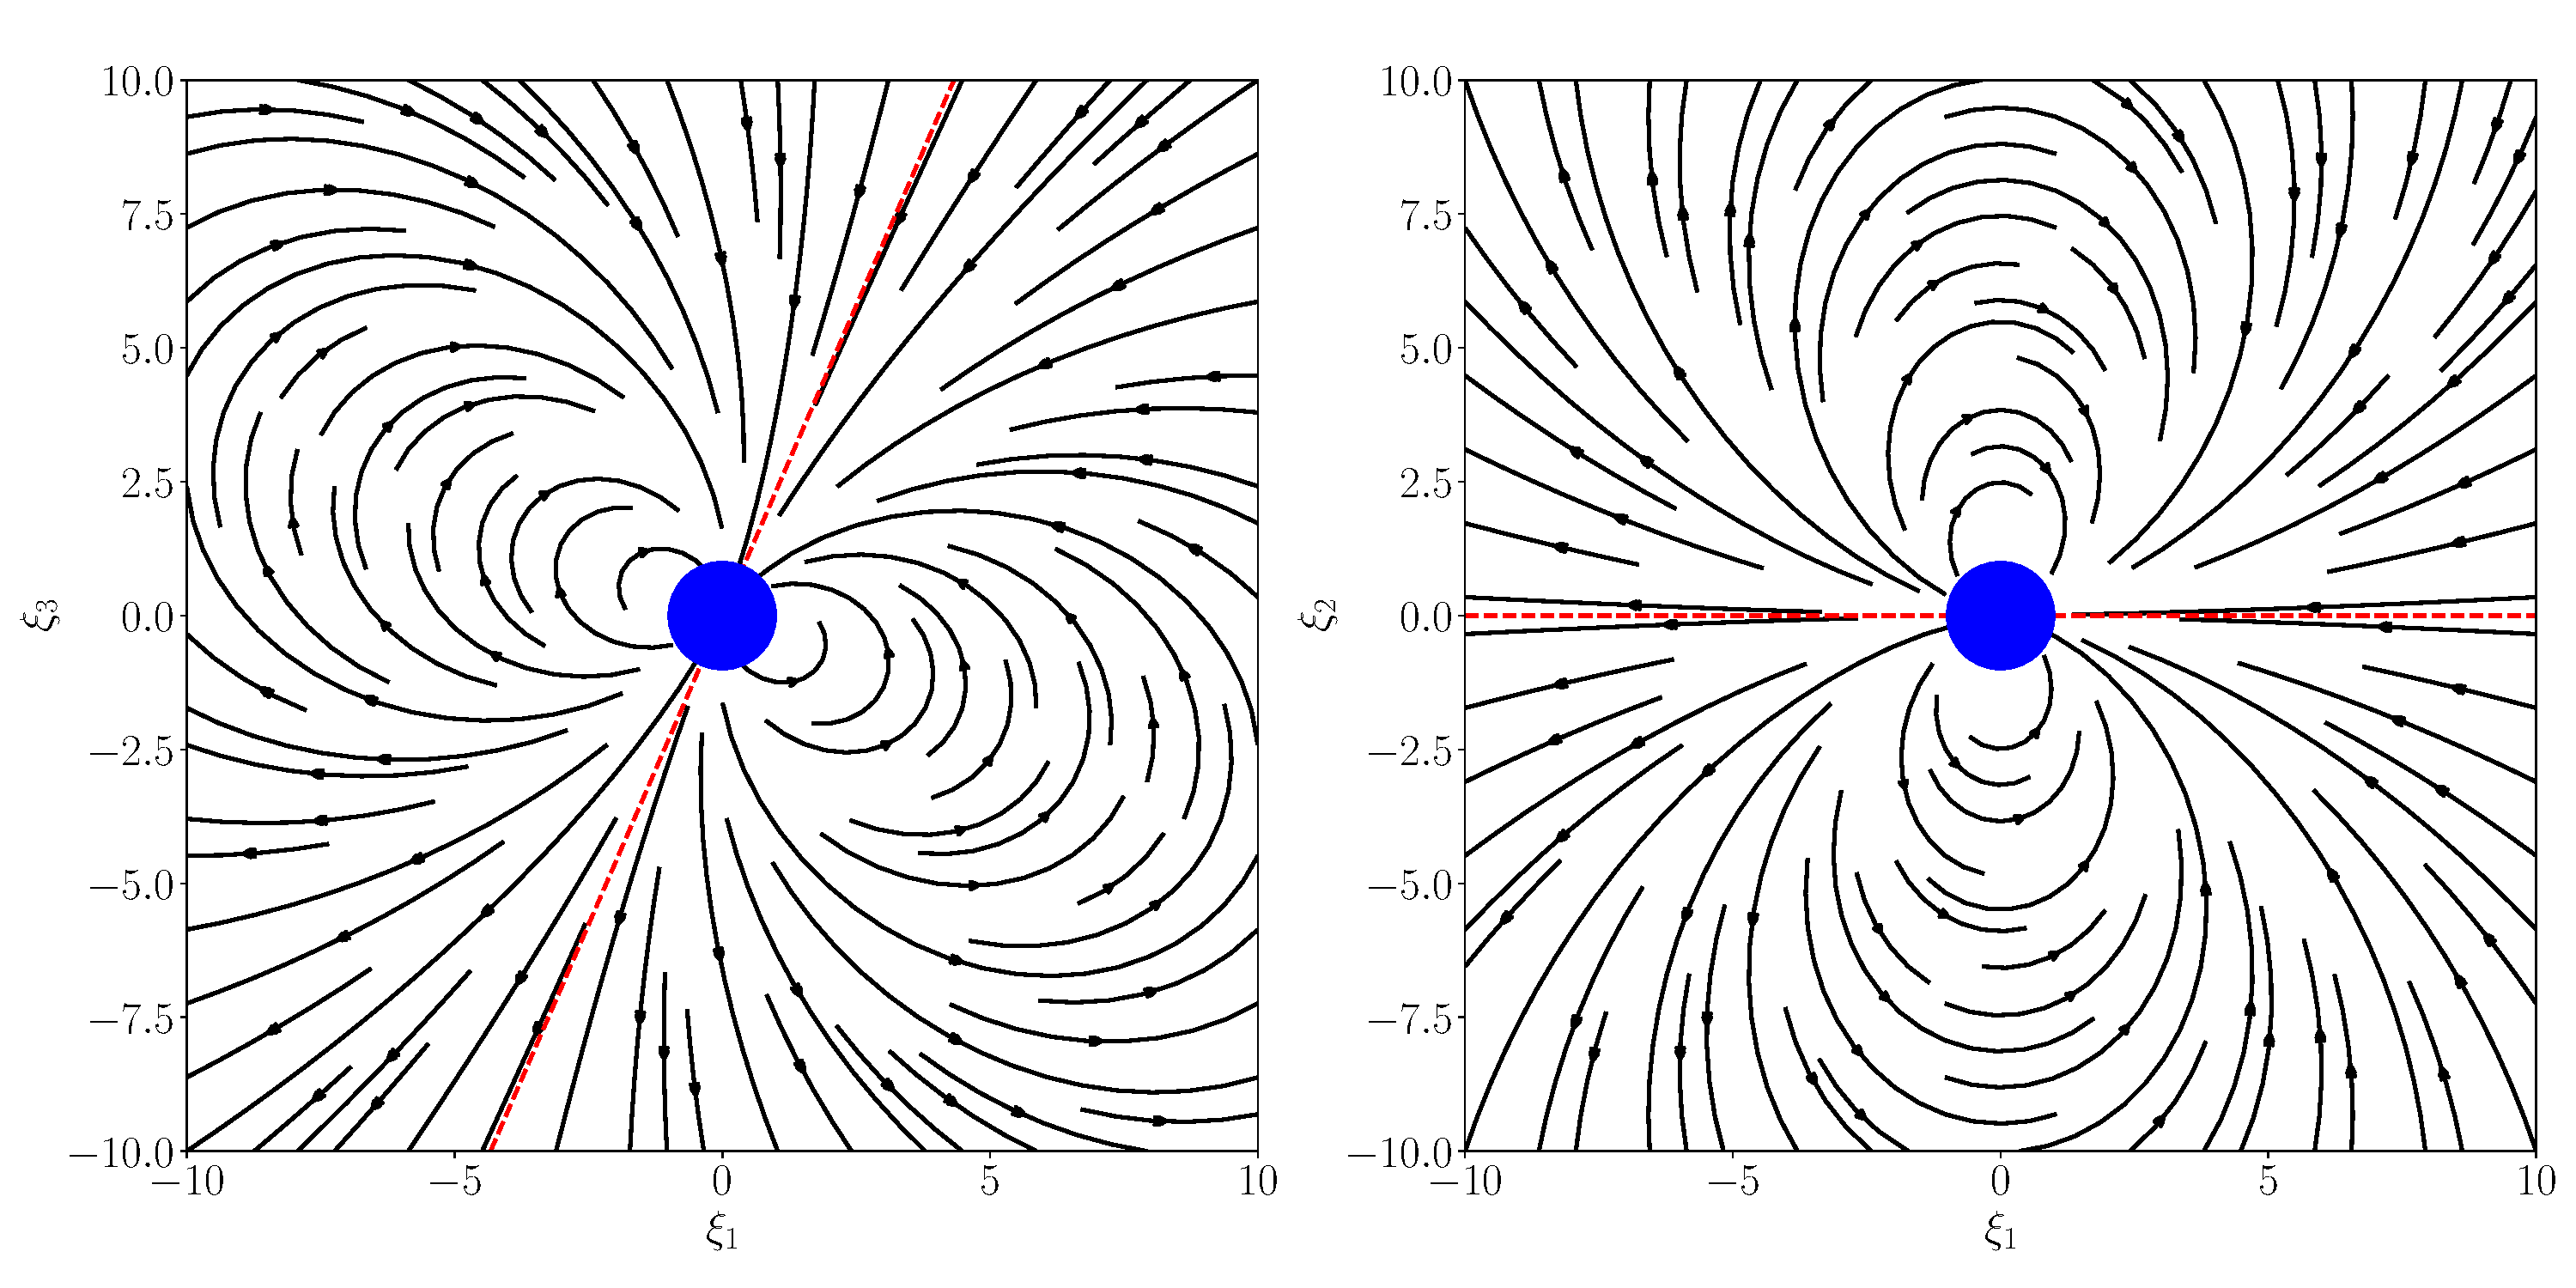
\includegraphics[width=\columnwidth]{../fig/earth.pdf}
	\caption{Magnetic field from earth. The tilt of the ecliptic with respect to the equator is $23.5^\circ$ \cite{https://doi.org/10.1029/2012JA018056}.}
	\label{fig:earth}
\end{figure}

When sending particles far from the earth towards it they start spiralling around the field lines. This is consistent with the fact that the magnetic force acts perpendicular to the trajectory, and the fact that the motion along $\mathbf{B}$ is uniform in the first approximation, as considered in section \ref{sec:motion}. This is shown in figure \ref{fig:fast_part} and \ref{fig:slow_part}. 
%Also apparent from these plots is that the gyration radius is larger when the particles are sent towards earth with larger speed. 
Moreover, in figure \ref{fig:fast_part} we observe a clockwise drift around the equator, as predicted by equation \eqref{eq:v_grad} and \eqref{eq:v_curv}.

\begin{figure}[h!]
	\centering
	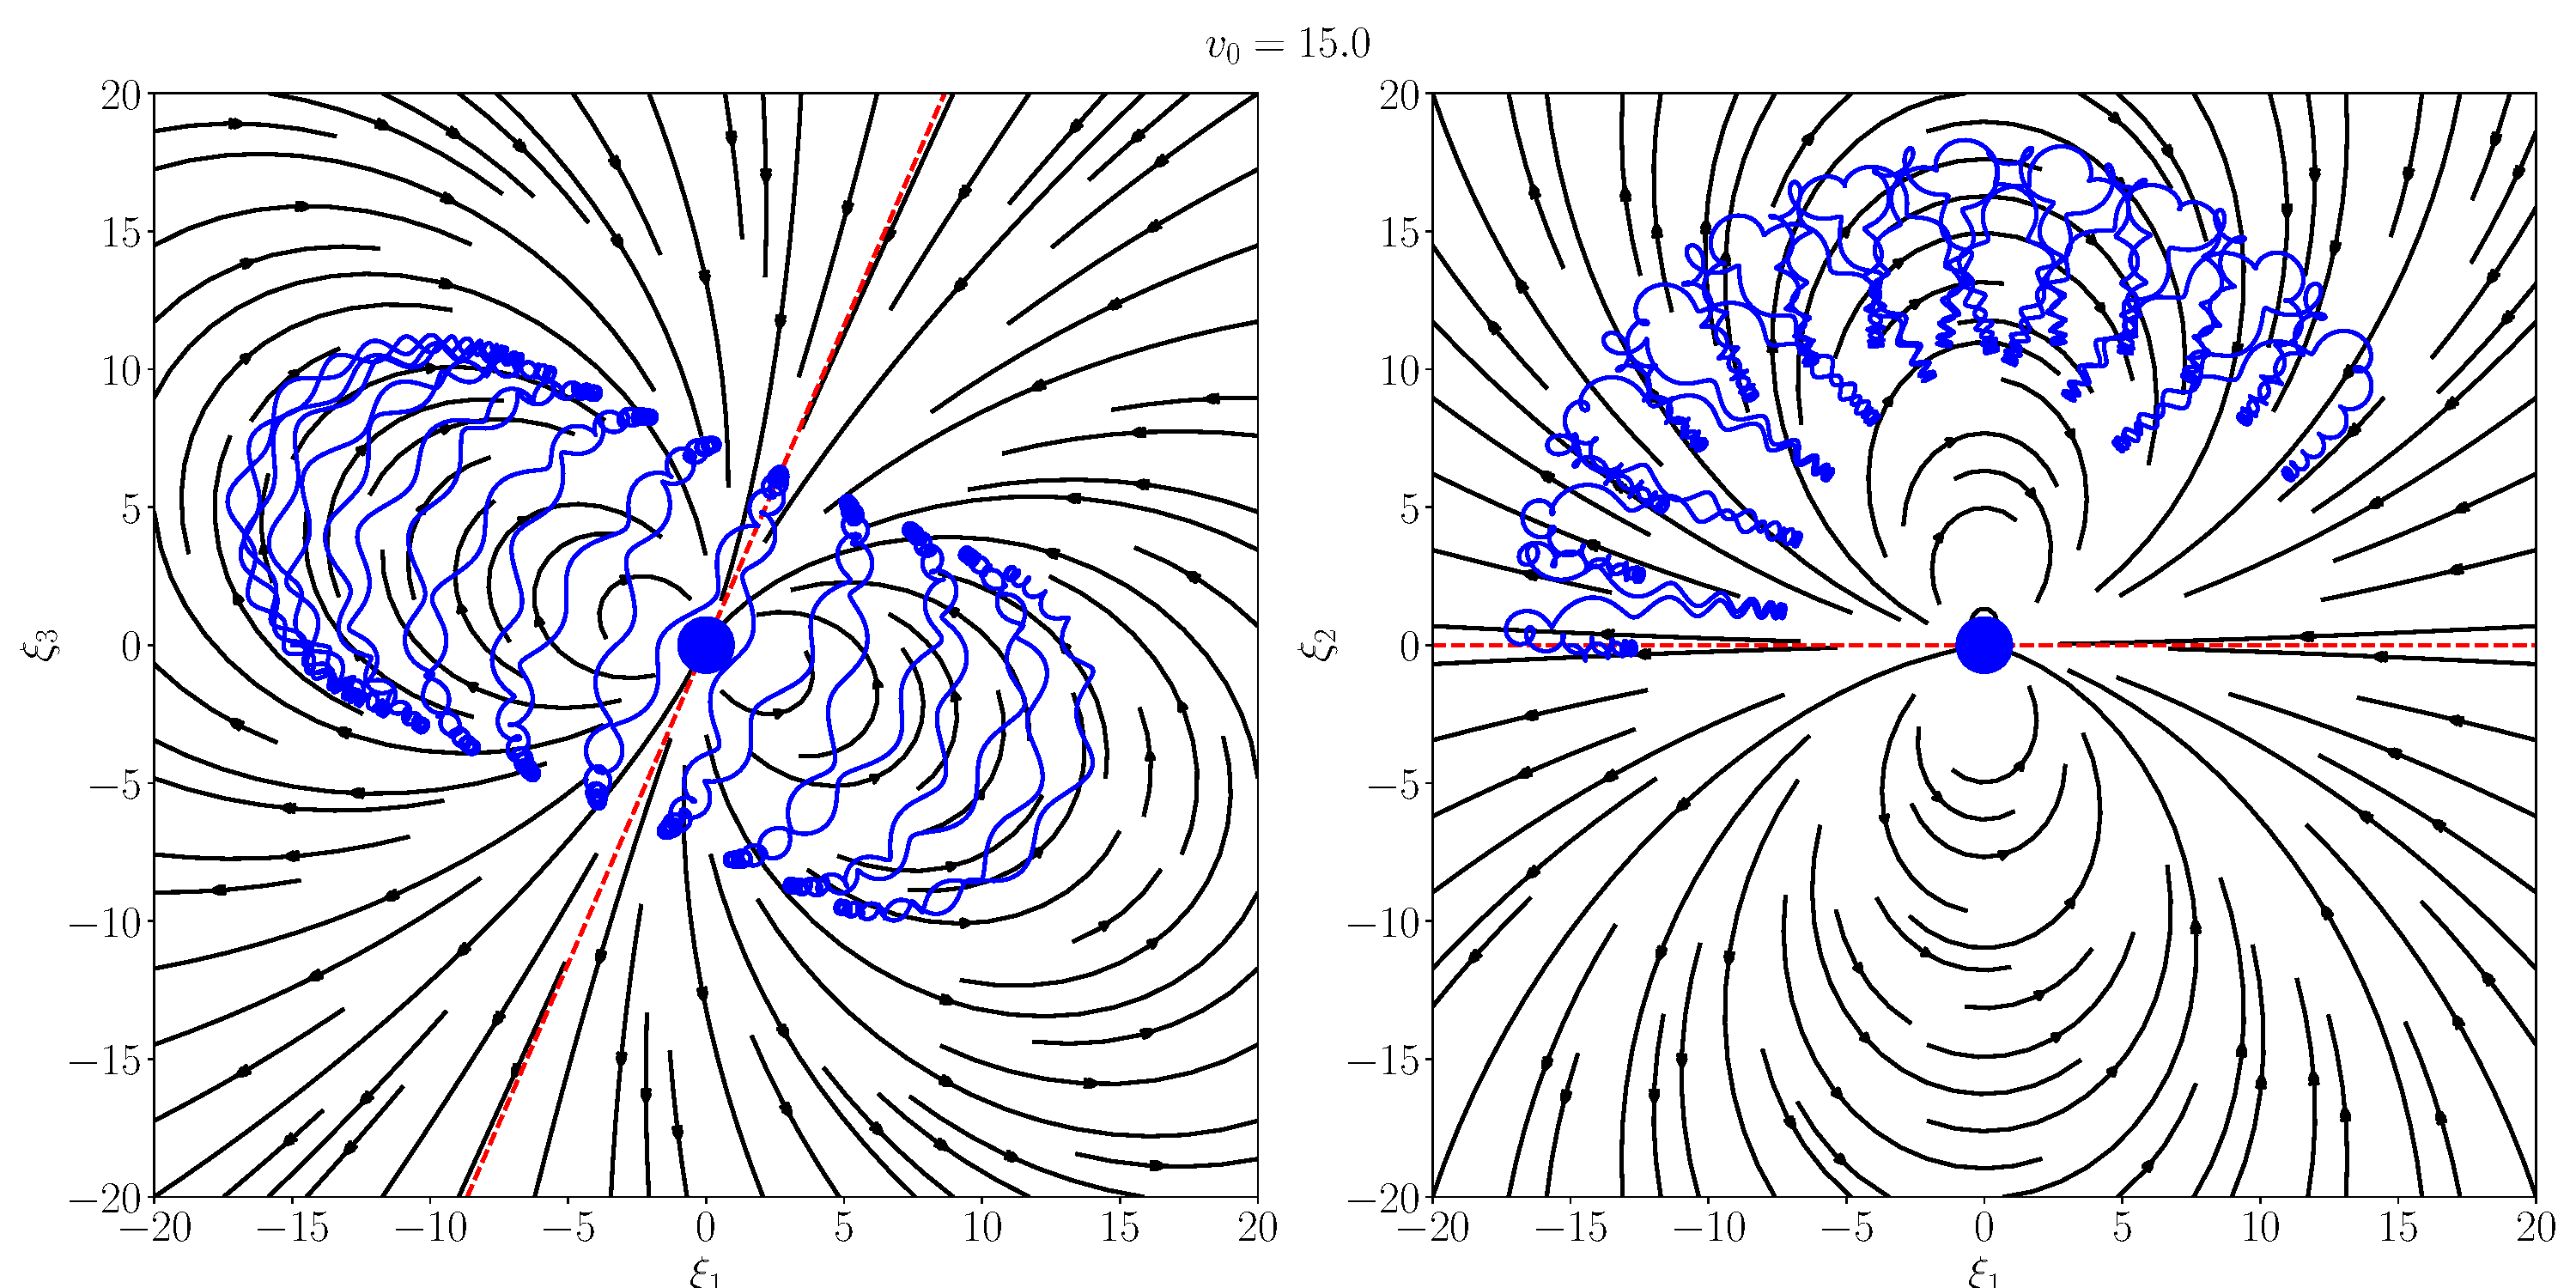
\includegraphics[width=\columnwidth]{../fig/earth_traj_fast.pdf}
	\caption{Particle sent towards the earth with high solar wind velocity.}
	\label{fig:fast_part}
\end{figure}

The trajectories of particles sent towards earth at different heights $z$ ($\xi_3$) is shown in figure \ref{fig:different_z}.

\begin{figure}[htb]
	\centering
	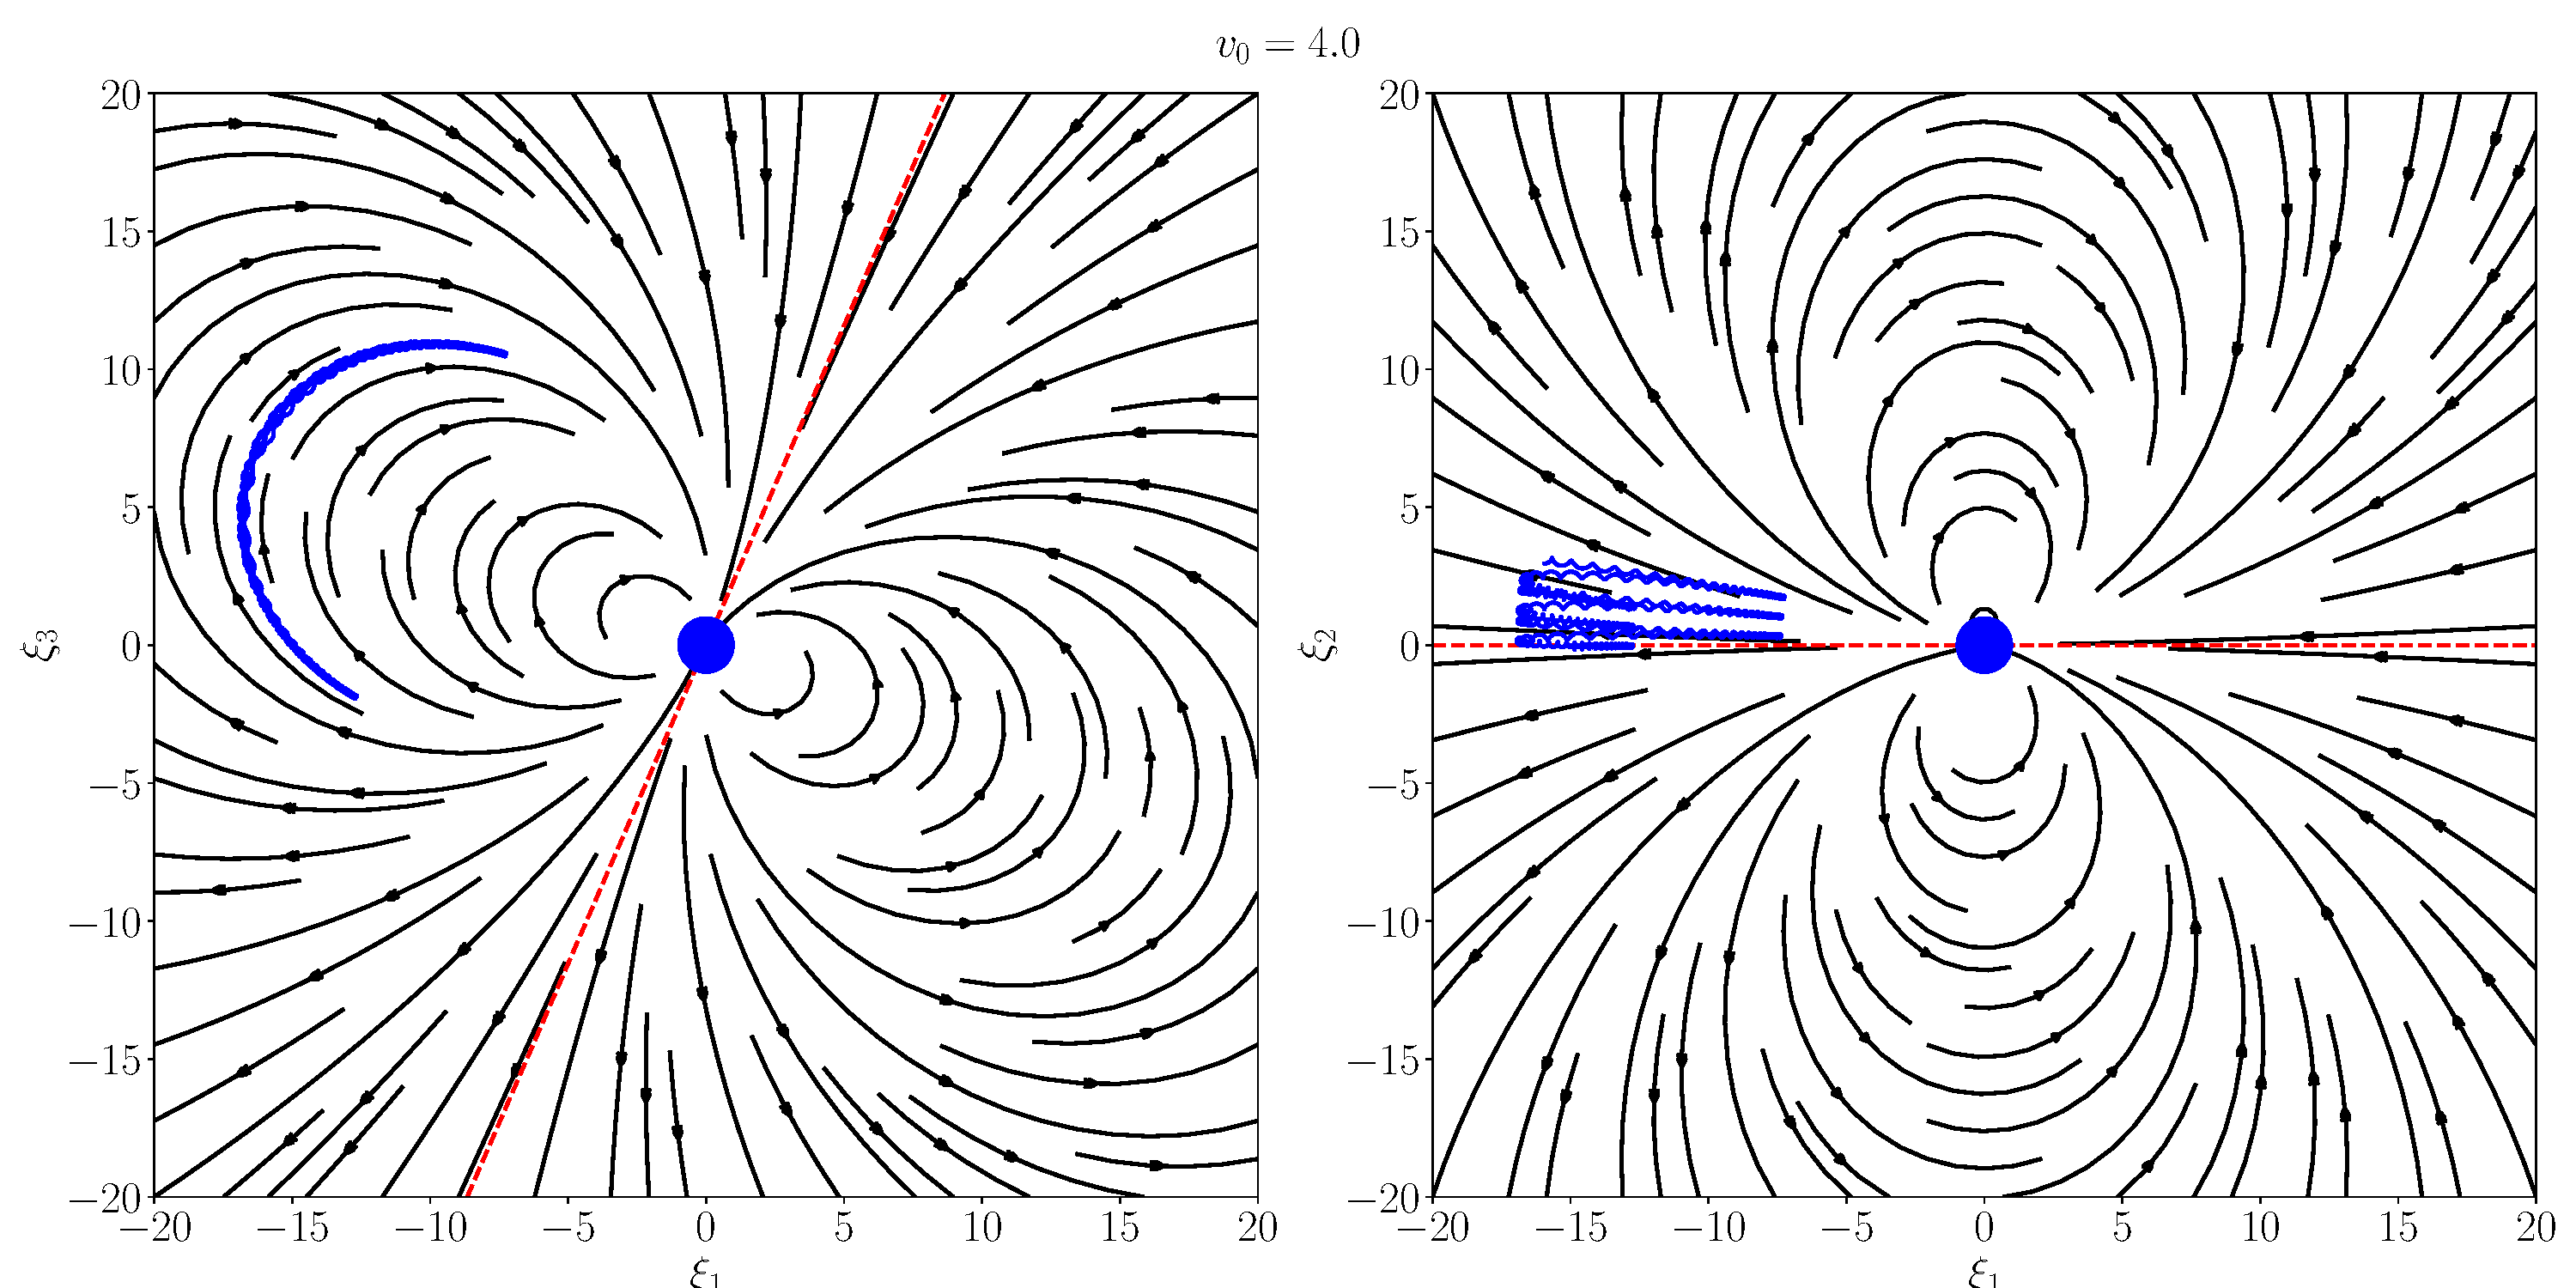
\includegraphics[width=\columnwidth]{../fig/earth_traj_slow.pdf}
	\caption{Particle sent towards the earth with typical solar wind velocity.}
	\label{fig:slow_part}
\end{figure}
\begin{figure}[h!]
	\centering
	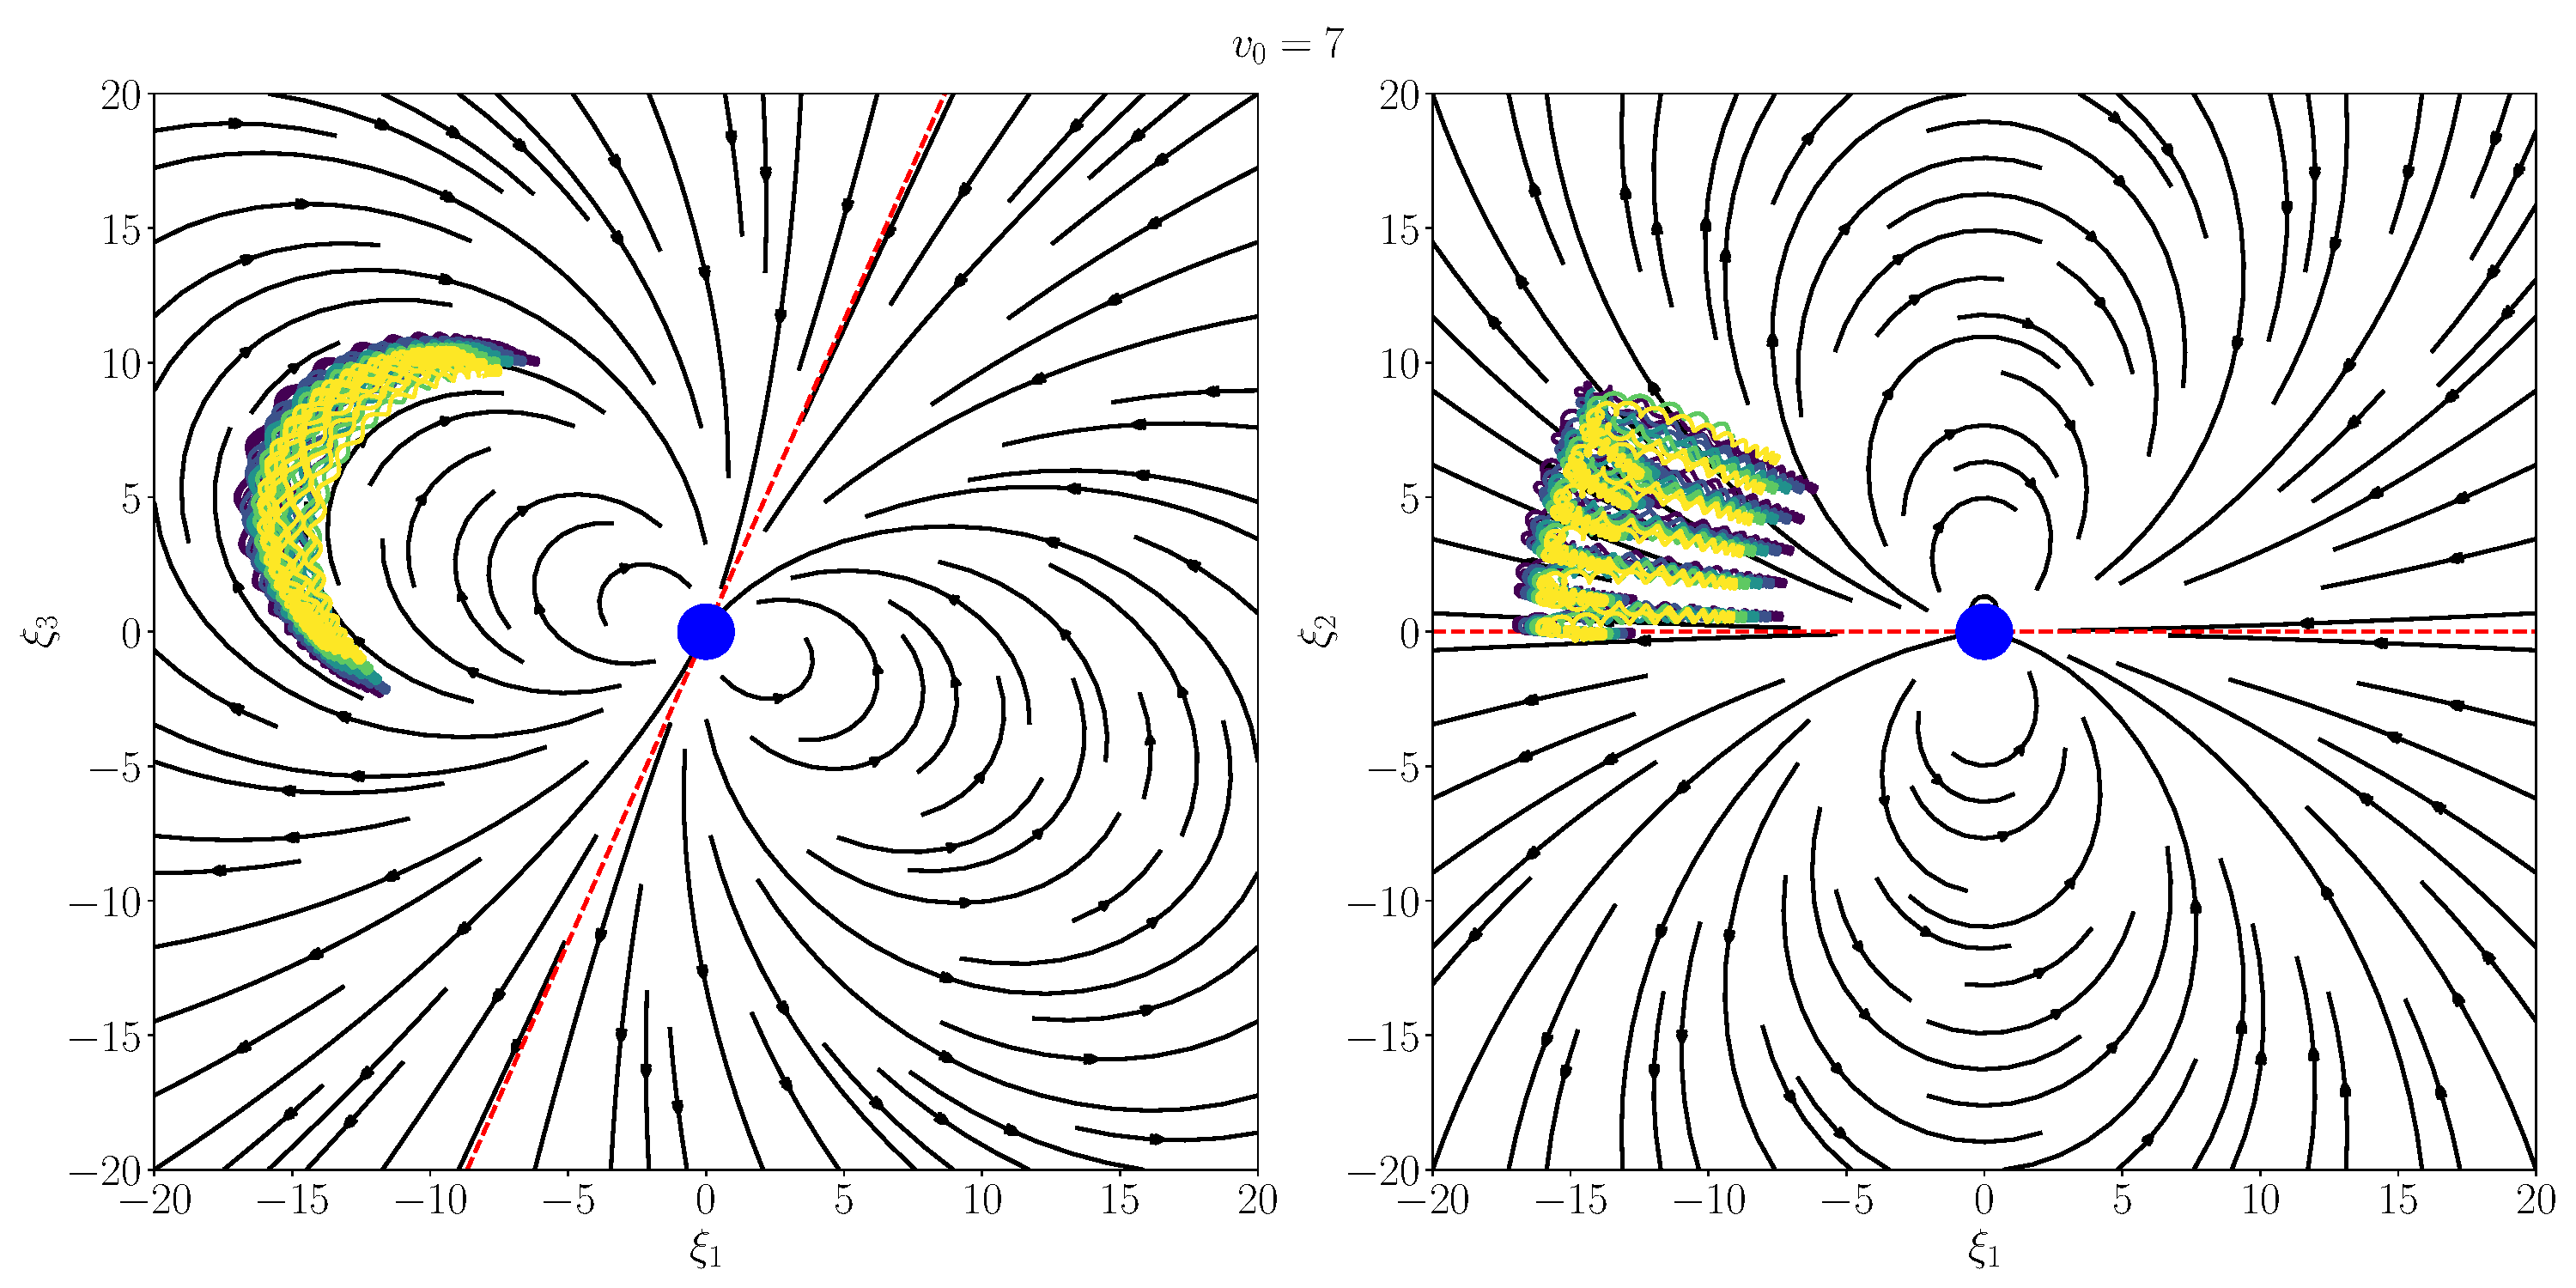
\includegraphics[width=\columnwidth]{../fig/traj_diffz.pdf}
	\caption{Particle sent towards the earth with typical solar wind velocity, for different heights $z_0$.}
	\label{fig:different_z}
\end{figure}

When doing this exact same simulation but with a weaker field ($\hat{B} \to 1/100 \hat{B}$) we observe that the same qualitative behaviour is captured. Moreover, we see here more clearly that the particles tend to spiral in towards the poles. This is exactly what causes the Aurora to be visible here and not near the equator. Note however that the strength of this field has nothing to do with that of earth's, so this demonstration is therefore not to be taken too seriously.

\begin{figure}[htb]
	\centering
	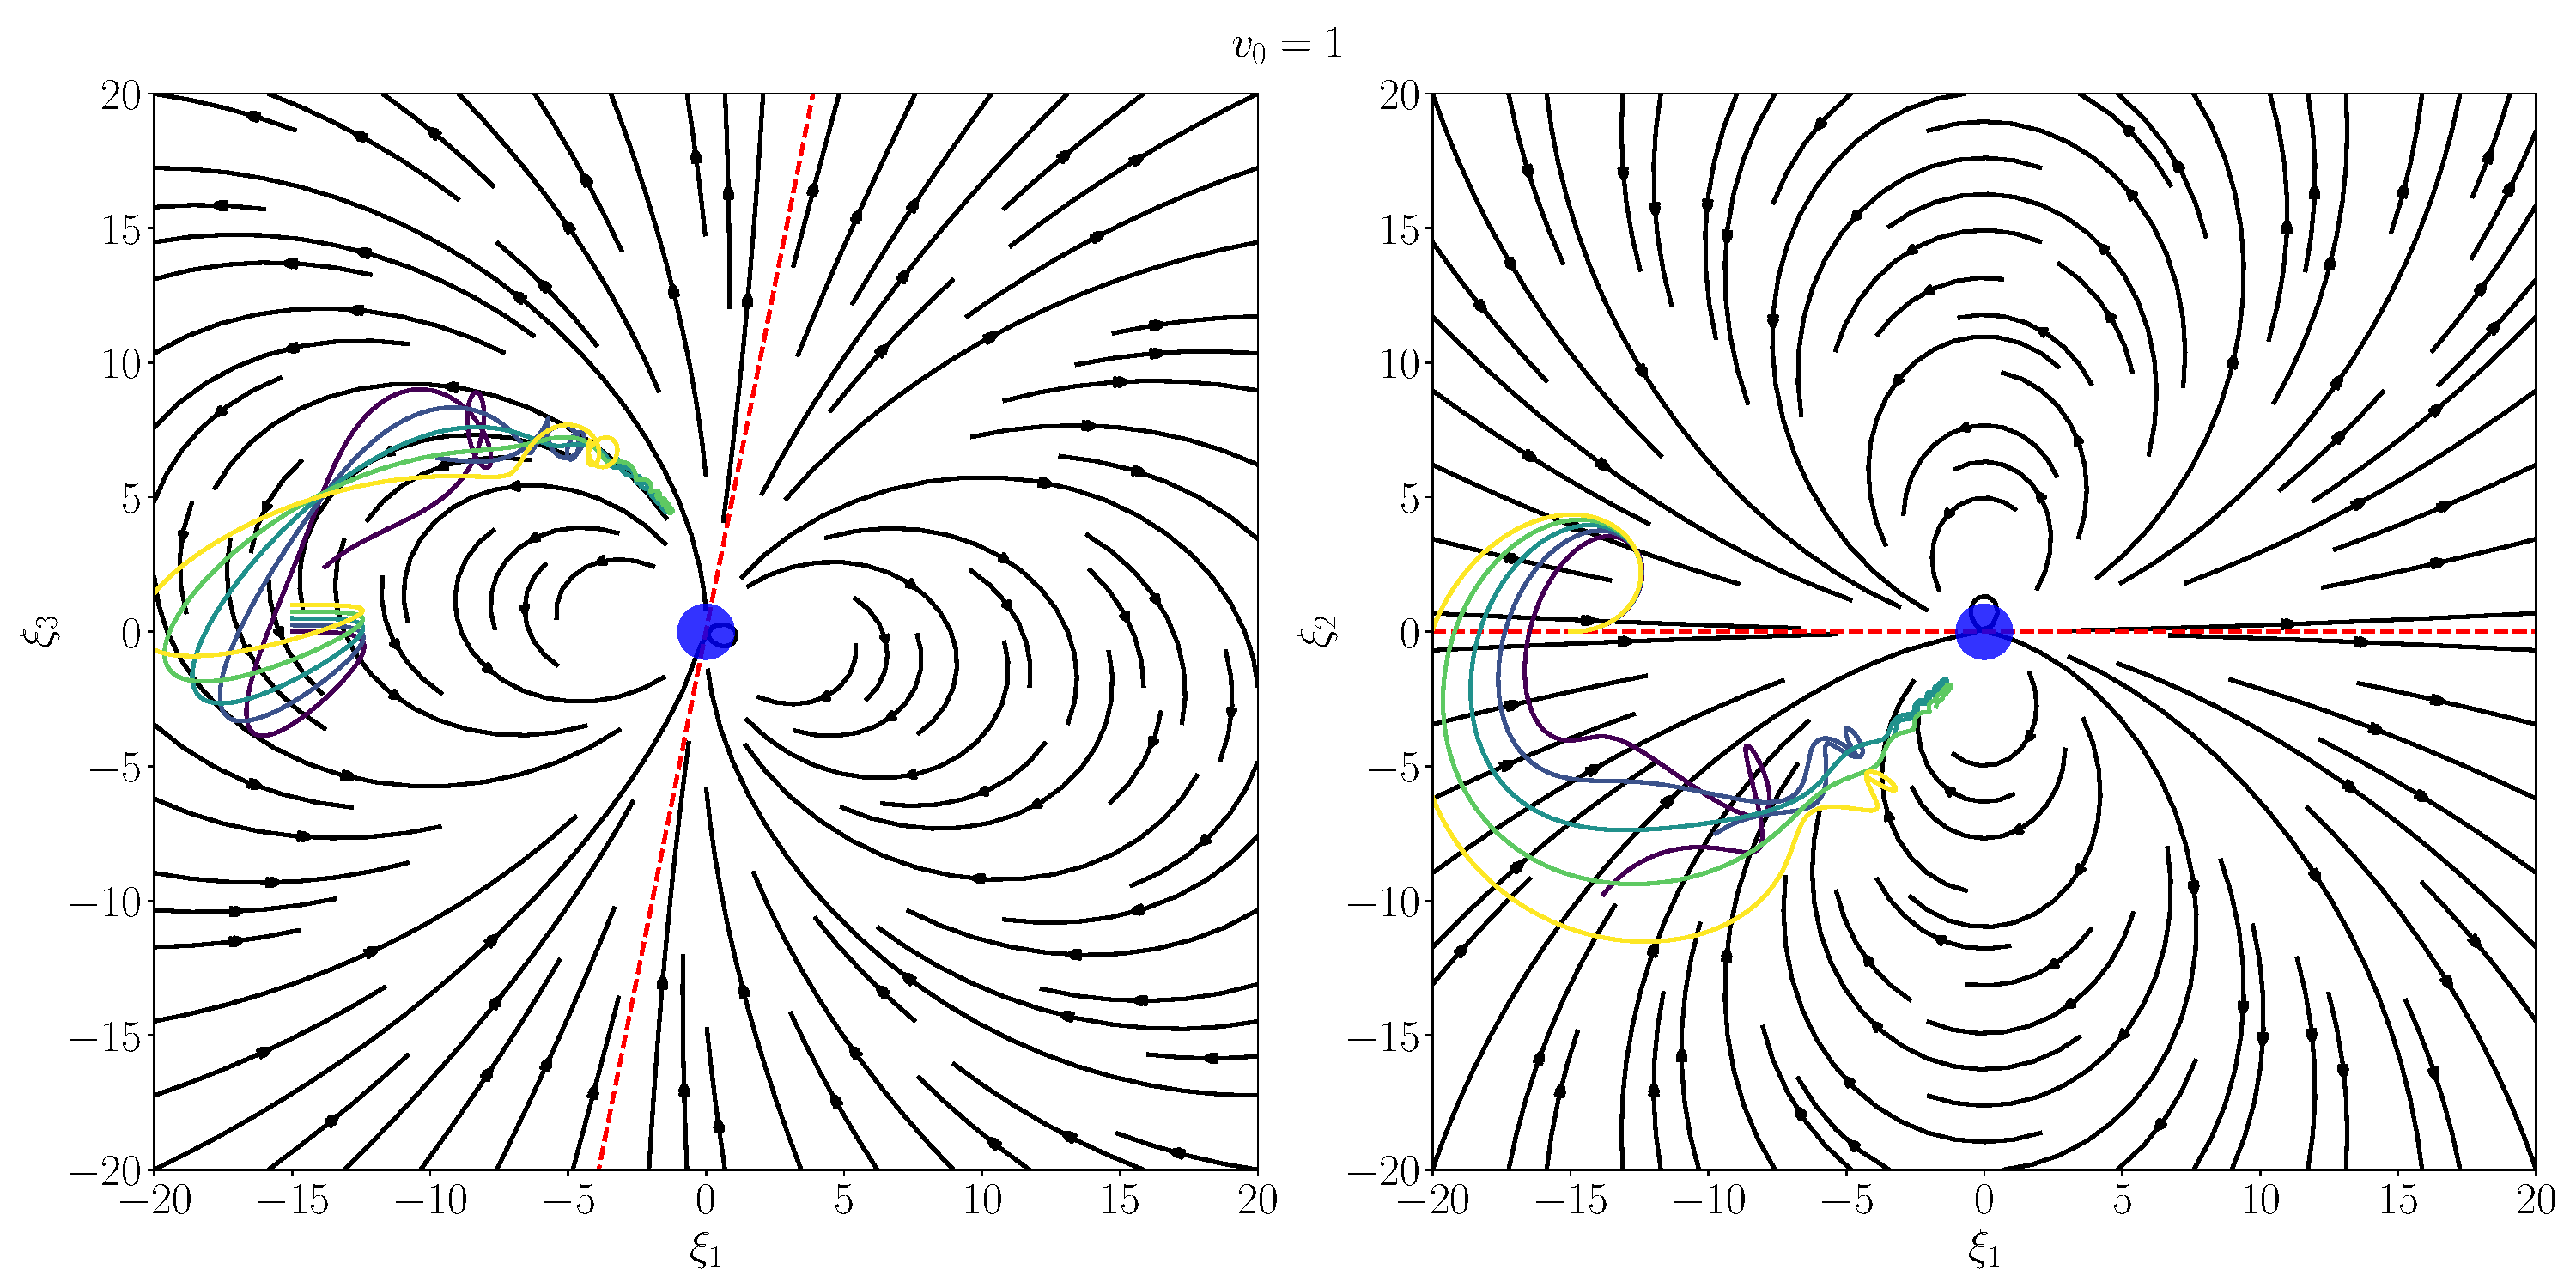
\includegraphics[width=\columnwidth]{../fig/weak_traj_diffz.pdf}
	\caption{Particle sent towards the earth with lower typical solar wind velocity, for different heights $z_0$, with a weaker field.}
	\label{fig:weak_different_z}
\end{figure}

\subsection{Validity of solution}

To have an idea of how good the numerical solution is we investigate how well energy is conserved for the particles. Since magnetic forces do no work, the energy should be invariant. The (normalised) energy difference as a function of time is shown in figure \ref{fig:energy} for some of the paths plotted above.

\begin{figure}[htb]
	\centering
	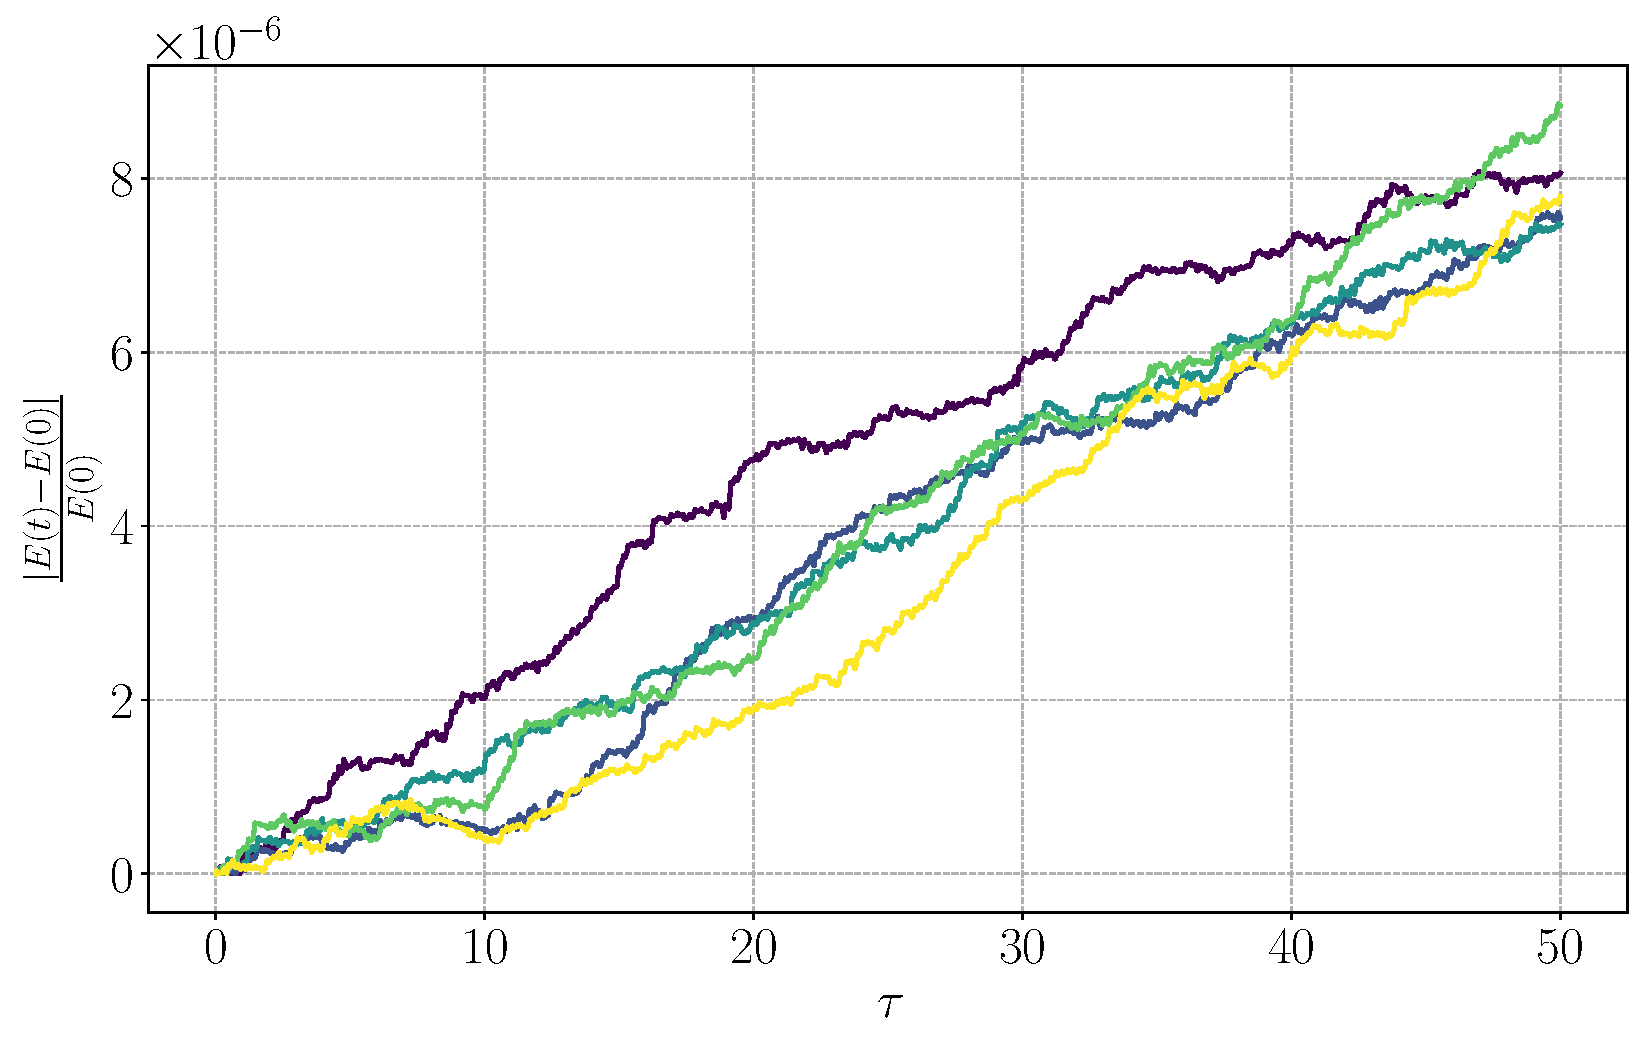
\includegraphics[width=0.8\columnwidth]{../fig/energy.pdf}
	\caption{Energy difference as a function of time for the $5$ trajectories shown in figure \ref{fig:different_z}.}
	\label{fig:energy}
\end{figure}

As the variations in the energy shown in figure \ref{fig:energy} are $\ll 1$ we conclude that the numerical validity of the solutions are good. There is however a slight drift in the energy, but that is inevitable when we take into consideration numerical round-off errors. 
 
\section{Conclusion}

Despite the fact that the model used is extremely simple, it captures the essence of the physics involved. The plots show that the particles are trapped in helical trajectories following the field lines, exactly as one would predict using electromagnetic theory. 

Moreover, through modifying the parameters of the model slightly, the particles are shown to be spiralling in towards the poles. This is in accordance with the fact that the Aurora is observed here. However, this fact is based on a rather flimsy demonstration, as special relativity starts playing an important role when the energy of the particles increases this much.

A more careful analysis is needed to include the relativistic corrections to the trajectories. This is not embarked on here. 



\bibliographystyle{alpha}
\bibliography{references}

\end{document}